\documentclass{article}

\usepackage{url,fullpage,amsmath,amssymb,graphicx}
\graphicspath{{Fig/}}

\def\Poincare{\mathrm{Poincar\acute{e}}}
\def\Hilbert{\mathrm{Hilbert}}
\def\Sym{\mathrm{Sym}}
\def\Log{{\mathrm{Log}}}
\def\barS{\bar{S}}
\def\det{\mathrm{det}}
\def\dsigma{\mathrm{d}\sigma}
\def\hatP{{\hat{P}}}
\def\Sinh{\mathrm{Sinh}}
\def\Cosh{\mathrm{Cosh}}
\def\sinh{\mathrm{sinh}}
\def\cosh{\mathrm{cosh}}
\def\arccsch{\mathrm{arccsch}}
\def\arccosh{\mathrm{arccosh}}
\def\arcsinh{\mathrm{arcsinh}}
\def\arctanh{\mathrm{arctanh}}
\def\bbP{\mathbb{P}}
\def\FR{\mathrm{FR}}
\def\SSPD{\mathrm{SSPD}}
\def\RieSEB{\mathrm{RieSEB}}
\def\calS{\mathcal{S}}
\def\calD{\mathcal{D}}
\def\supp{\mathrm{supp}}
\def\ball{\mathrm{ball}}
\def\calM{\mathcal{M}}
\def\calG{\mathcal{G}}
\def\SH{\mathbb{SH}}
\def\Sym{\mathrm{Sym}}
\def\dZ{\mathrm{d}Z}
\def\dY{\mathrm{d}Y}
\def\dP{\mathrm{d}P}
\def\dZbar{\mathrm{d}\bar Z}
\def\barZ{{\bar{Z}}}
\def\dtheta{\mathrm{d}\theta}
\def\SPC{\mathrm{SPC}}
\def\trace{\mathrm{trace}}
\def\proj{\mathrm{proj}}
\def\barN{{\overline{\mathcal{N}}}}
\def\dP{\mathrm{d}P}
\def\CO{\mathrm{CO}}
\def\bTheta{\bm{\Theta}}
\def\bEta{\mathbf{H}}
\def\rhoCO{\rho_{CO}}
\def\MVNSPD{C\&O\ }
\def\GL{\mathrm{GL}}
\def\KL{\mathrm{KL}}
\def\cN{\mathrm{cN}}
\def\Killing{\mathrm{Killing}}
\def\diag{\mathrm{diag}}
\def\CC{c}
\def\MVN{\mathrm{MVN}}
\def\SPD{\mathrm{SPD}}
\def\Aff{\mathrm{Aff}}
\def\bbR{\mathbb{R}}
\def\Fisher{\mathrm{Fisher}}
\def\vectortwo#1#2{{\left[\begin{array}{l}#1 \cr #2\end{array}\right]}}
\def\mattwotwo#1#2#3#4{{\left[\begin{array}{ll}#1 & #2\cr #3 & #4\end{array}\right]}}
\def\tr{\mathrm{tr}}
\def\barF{{\bar F}}
\def\bartheta{{\bar \theta}}
\def\bareta{{\bar \eta}}
\def\innerat#1#2#3{ {{\langle #2, #3\rangle}_{#1}} }
\def\inner#1#2{{\langle #1, #2\rangle}}
\def\calN{\mathcal{N}}
\def\Bi{\mathrm{Bi}}
\def\dx{\mathrm{d}x}
\def\dy{\mathrm{d}y}
\def\SPD{\mathrm{SPD}}
\def\calP{\mathcal{P}}
 \def\Rao{\mathrm{Rao}}
\def\Length{\mathrm{Length}}
\def\dt{\mathrm{d}t}
\def\rhoN{\rho_{\calN}}
\def\rhoP{\rho_P}
\def\mfdN{\mathscr{N}}
\def\mfdbarP{\bar\mathscr{P}}
\def\SS{\mathrm{SS}}
\def\dbeta{\mathrm{d}\beta}
\def\barLambda{{\bar\Lambda}}
\def\mfdP{\mathscr{P}}
\def\dim{\mathrm{dim}}
\def\Aff{\mathrm{Aff}}
\def\Var{\mathrm{Var}}
\def\vech{\mathrm{vech}}
\def\std{\mathrm{std}}
\def\barC{{\bar C}}
\def\barP{{\bar P}}
\def\dSigma{\mathrm{d}\Sigma}
\def\dmu{\mathrm{d}\mu}
\def\ds{\mathrm{d}s}
\def\st{\ :\ }
\def\bbR{\mathbb{R}}
\def\nablaG{\stackrel{\mathscr{G}}{\nabla}}
\def\nablaP{\stackrel{\mathscr{P}}{\nabla}}
\def\nablacG{\stackrel{\mathscr{G}_0}{\nabla}}
\def\Cov{\mathrm{Cov}}
\def\SL{\mathrm{SL}}
\def\SO{\mathrm{SO}}
\def\CandO{{C\&O}}


\title{A Simple Approximation Method for the Fisher-Rao Distance between Multivariate Normal Distributions}
\author{Frank Nielsen}
\date{2023}

\begin{document}
\maketitle


\section{The Fisher-Rao distance}

Let $\bbP(d)$ denote the set of symmetric positive?definite (SPD) $d\times d$ matrices and $\calN(d)$ denote 
the set of multivariate normal distributions:

$$
\calN(d):=\left\{p_{\mu,\Sigma}(x)= (2\pi)^{^\frac{d}{2}} |\Sigma|^{-\frac{1}{2}} \exp\left(-\frac{1}{2}(x-\mu)^\top\Sigma^{-1}(x-\mu)\right) 
\st   (\mu,\Sigma)\in\Lambda(d):=\bbR^d\times \bbP(d)
\right\},
$$


The Fisher-Rao distance between two normals $N(\mu_1,\Sigma_1)$ and $N(\mu_2,\Sigma_2)$ is the geodesic Riemannian distance on the manifold $(\calN,g^\Fisher)$ induced by the Fisher information metric:

$$
\rho_\calN(N(\lambda_1),N(\lambda_2)):=\inf_{\substack{c(t)\\ c(0)=p_{\lambda_1}\\ c(1)=p_{\lambda_2}}}  \, \left\{\Length(c)\right\},
$$
\noindent where 
$$
\Length(c):=\int_0^1  \ds^\Fisher(c(t)) \dt,
$$
and $\ds^\Fisher(t):=\sqrt{\inner{\dot c(t)}{\dot c(t)}}_{c(t)}$ is the Fisher-Rao length element.
The inner product $\inner{v_1}{v_2}_{N}$ for $v_1,v_2\in T_N\calN$ at normal $N$ is the called the Fisher-Rao norm (with tangent planes $T_N\calN$ is identified  to $\bbR^d\times\Sym(d)$ where $\Sym(d)$ be the set of $d\times d$ symmetric matrices).
The statistical model $\calN(d)$ is of dimension $m=\dim(\Lambda(d))=d+\frac{d(d+1)}{2}=\frac{d(d+3)}{2}$ and identifiable:
there is a one-to-one correspondence $\lambda \leftrightarrow p_\lambda(x)$ between $\lambda\in\Lambda(d)$ and $N(\mu,\Sigma)\in\calN(d)$.

\begin{itemize}

\item When $d=1$, the Fisher-Rao distance is known in closed form:
$$
\rho_{\calN}(N_1,N_2)= 2\sqrt{2}\,\arctanh(\Delta(\mu_1,\sigma_1;\mu_2,\sigma_2)),
$$
where $\Delta(a,b;c,d)=\sqrt{\frac{(c-a)^2+2(d-b)^2}{(c-a)^2+2(d+b)^2}}$ is a M\"obius distance and $\arctanh(u):=\frac{1}{2}\log\left(\frac{1+u}{1-u}\right)$ for $0\leq u<1$.
The Fisher?Rao geodesics are semi-ellipses with centers located on the $x$-axis:

\begin{center}
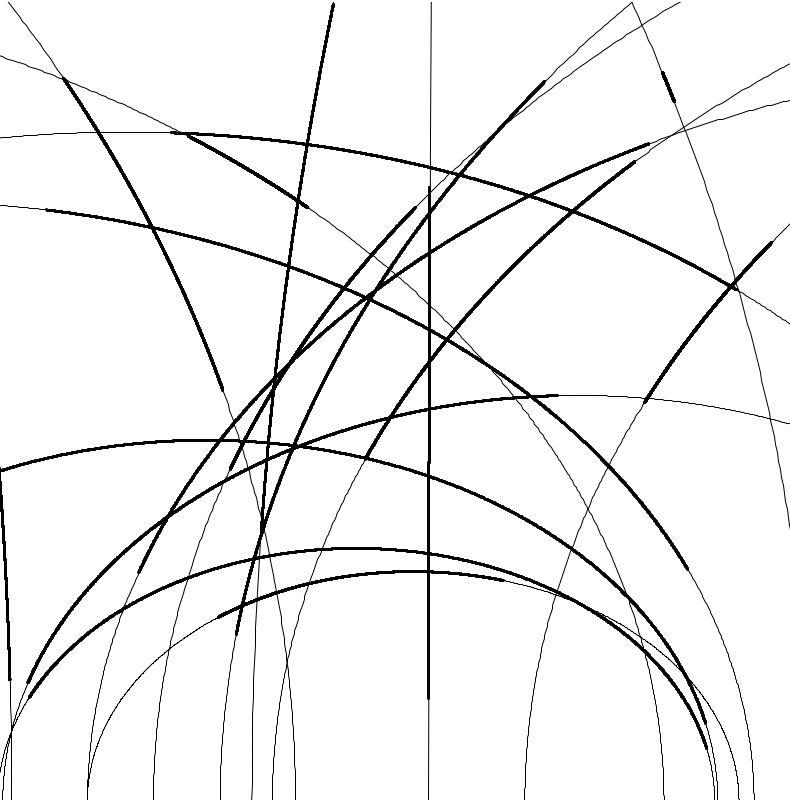
\includegraphics[width=0.4\textwidth]{FisherRaoGeodesics1D.png} 
\end{center}

\item When the normal distributions belongs to the same submodel $\calN_\mu=\{N(\mu,\Sigma)\st \Sigma\in\calP(d)\}\subset\calN$ of normal distributions sharing the same mean $\mu$, we have~\cite{DoubleCone-James-1973,Skovgaard-1984}:  
\begin{eqnarray*}
\rho_{\calN_\mu}(N_1,N_2)&=& \sqrt{\frac{1}{2} \sum_{i=1}^d \log^2 \lambda_i(\Sigma_1^{-1}\Sigma_2)},
\end{eqnarray*}
where $\lambda_i(M)$ denotes the $i$-th generalized largest eigenvalue of matrix $M$, where the generalized eigenvalues are solutions of the equation $|\Sigma_1-\lambda\Sigma_2|=0$. The submanifold $(\calN_\mu,g^\Fisher)$ is totally geodesic in $(\calN,g^\Fisher)$.

\item When the normal distributions belongs to the same submodel 
$\calN_\Sigma=\{N(\mu,\Sigma)\st \Sigma\in\calP(d)\}\subset\calN$ of normal distributions sharing the same covariance matrix $\Sigma$
we have
$$
\sqrt{2}\, \arccosh\left(1+\frac{1}{4}\Delta_\Sigma^2(\mu_1,\mu_2)\right),
$$
where $\Delta_\Sigma$ is the Mahalanobis distance:
$$
\Delta_\Sigma(\mu_1,\mu_2):=\sqrt{(\mu_2-\mu_1)^\top \Sigma^{-1} (\mu_2-\mu_1)}.
$$
\end{itemize}

However, in the general case, the Fisher-Rao distance between normals is not known in closed form~\cite{FRMVNReview-2020}.

\section{Isometric embedding into the higher-dimensional SPD cone}

 
Calvo and Oller~\cite{SDPMVN-1990} show how to embed $N(\mu,\Sigma)\in\calN(d)= \left\{\barP=f_{\beta}(\mu,\Sigma) \st (\mu,\Sigma)\in \calN(d)=\bbR^d\times\calP(d)\right\}$ into a SPD matrix   of $\bbP(d+1)$:
$$
\barP(N)=f(N)=\mattwotwo{\Sigma+\mu\mu^\top}{\mu}{\mu^\top}{1}
$$ 
so that the manifold $(\calN(d),g^\Fisher)$ is isometrically embedded into the submanifold $(\barN,g^\trace)$ of the cone equipped with the trace metric
$$
g_P^\trace(P_1,P_2):= \frac{1}{2}\tr(P^{-1}P_1P^{-1}P_2).
$$
 
However, the submanifold $\barN\subset\bbP(d+1)$ is not totally geodesic.
Thus Calvo and Oller~\cite{SDPMVN-1990} derived a lower bound on the Fisher-Rao distance:
$$
\rho_\CO(N_1,N_2)=\sqrt{\frac{1}{2}}\, \sqrt{\frac{1}{2} \sum_{i=1}^d \log^2 \lambda_i(\barP_1^{-1}\barP_2)}
$$
which is also metric distance.


\section{A simple approximation method}

Our method consists in projecting the SPD geodesic $\gamma_{\bbP(d+1)}(\barP_1^{-1}\barP_2)$ onto $\barN$ and then maps back 
the SPD projected curve into $\calN$ by using $f^{-1}$: 
$$
c_\CO(N_1,N_2;t)=f^{-1}\left(\proj_{\barN}(\gamma_{\bbP(d+1)}(\barP_1^{-1}\barP_2;t))\right).
$$

Indeed, the geodesic $\gamma_{\bbP(d+1)}(\barP_1^{-1}\barP_2)$ has closed-form equation
$$
\gamma_{\bbP(d+1)}(\barP_1^{-1}\barP_2)=\barP_1^{\frac{1}{2}}\left(\barP_1^{-\frac{1}{2}}\barP_2\barP_1^{-\frac{1}{2}}\right)^t \barP_1^{\frac{1}{2}}.
$$

Now, we need to estimate the Fisher-Rao length of the curve $c_\CO(N_1,N_2;t)$ by discretizing the curve at $T$ positions:
$$
\tilde\rho_\CO(N_1,N_2)\leq \frac{1}{T} \sum_{i=1}^{T-1} \rho_\calN\left(c\left(\frac{i}{T}\right),c\left(\frac{i+1}{T}\right)\right), 
$$
and approximate for nearby normals their Fisher-Rao distances by the square root of their Jeffreys divergence:
$$
\rho_\calN\left(c\left(\frac{i}{T}\right),c\left(\frac{i+1}{T}\right)\right)\approx \sqrt{D_J\left[c\left(\frac{i}{T}\right),c\left(\frac{i+1}{T}\right)\right]},
$$
where
$$
D_J[p_{(\mu_1,\Sigma_1)}:p_{(\mu_2,\Sigma_2)}]=\tr\left(\frac{\Sigma_2^{-1}\Sigma_1+\Sigma_1^{-1}\Sigma_2}{2}-I\right)
+(\mu_2-\mu_1)^\top\frac{\Sigma_1^{-1}+\Sigma_2^{-1}}{2}(\mu_2-\mu_1).
$$

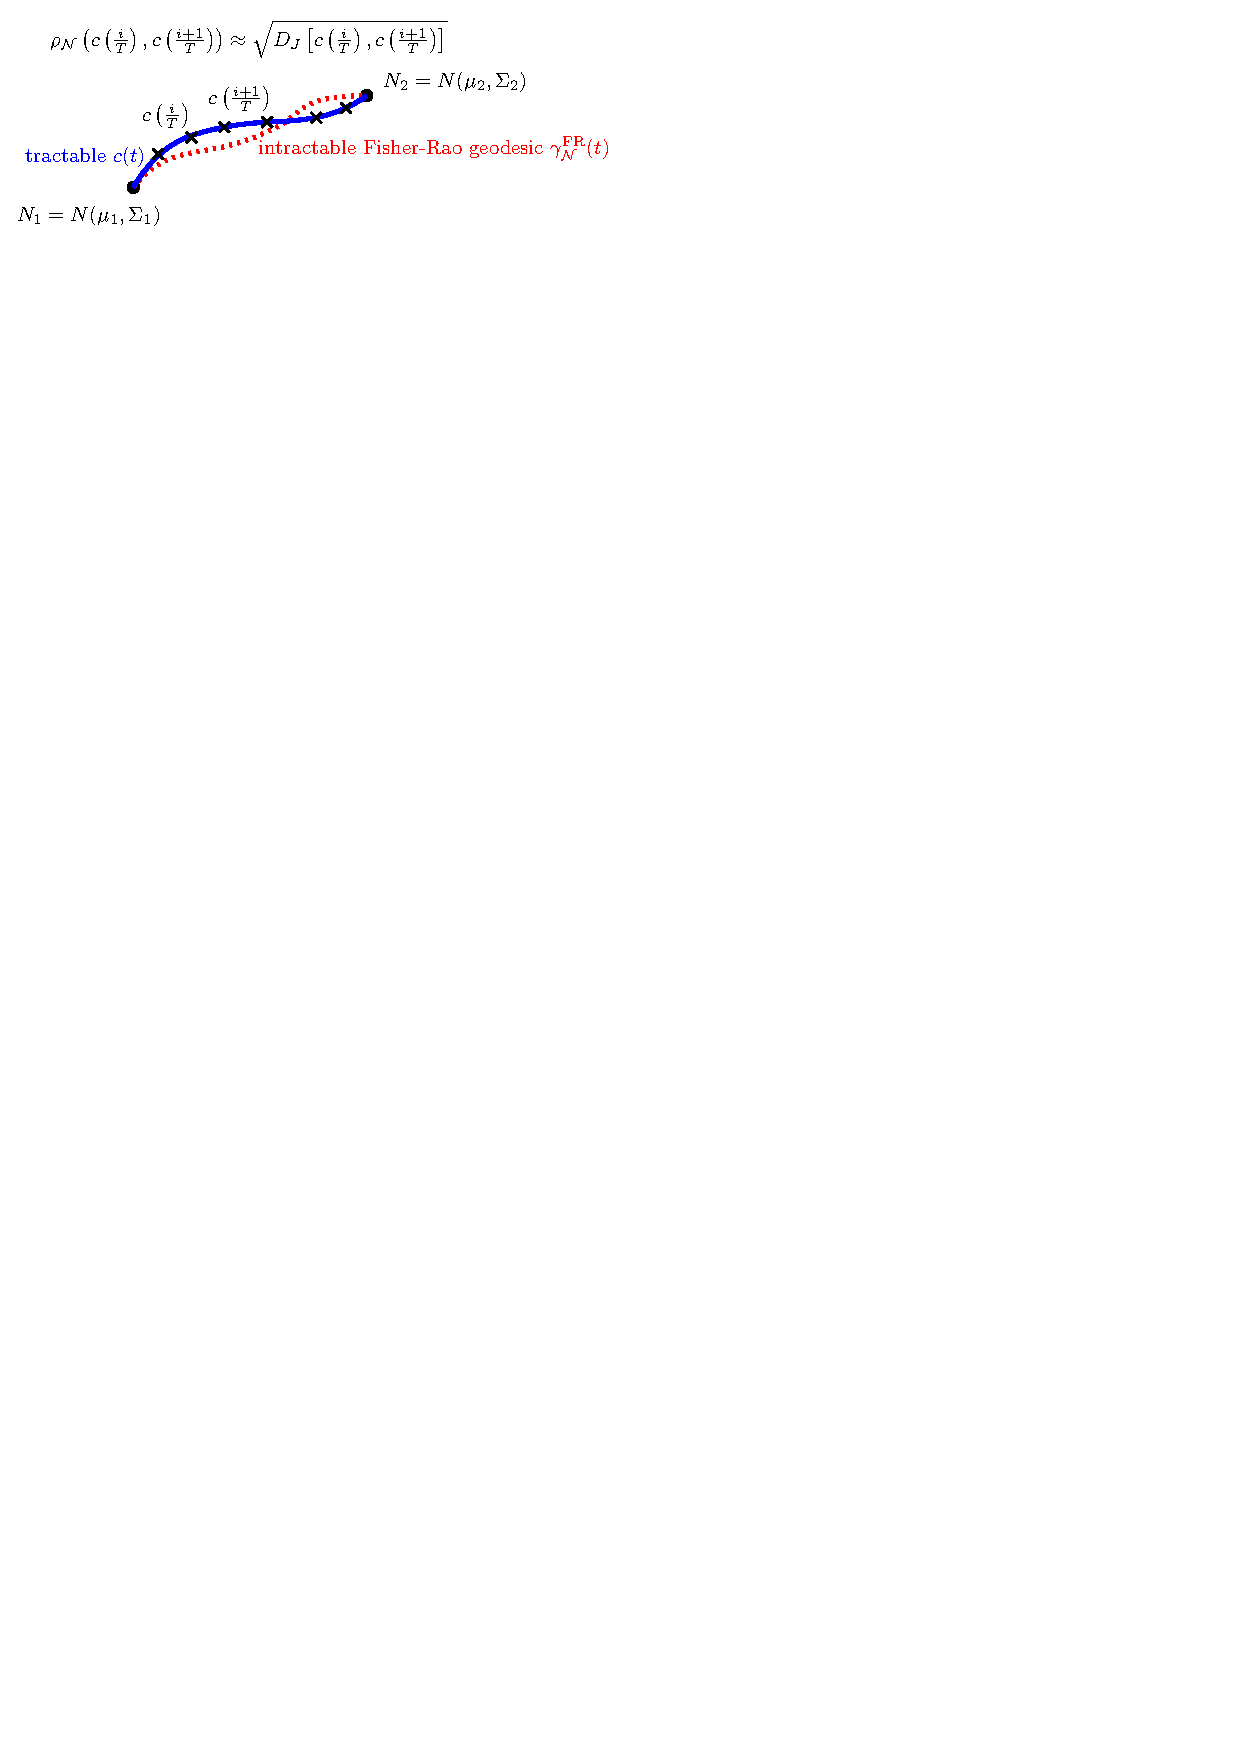
\includegraphics[width=0.8\textwidth]{FigIpe-ApproximationTractableCurve.pdf}

The projection of a SPD matrix $P\in\bbP(d+1)$ onto $\barN$ is done as follows:
Let $\beta=P_{d+1,d+1}$ and write  $P=\mattwotwo{\Sigma+\beta\mu\mu^\top}{\beta\mu}{\beta\mu^\top}{\beta}$.
Then the orthogonal projection at $P\in\calP$ onto $\barN$ is:
$$
\barP_\perp:=\proj_{\barN}(P)=\mattwotwo{\Sigma+\mu\mu^\top}{\mu^\top}{\mu}{1},
$$
and the SPD distance between $P$ and $\barP_\perp$  is
$$
\rho_\calP(P,\barP_\perp)=\frac{1}{\sqrt{2}} |\log\beta|.
$$

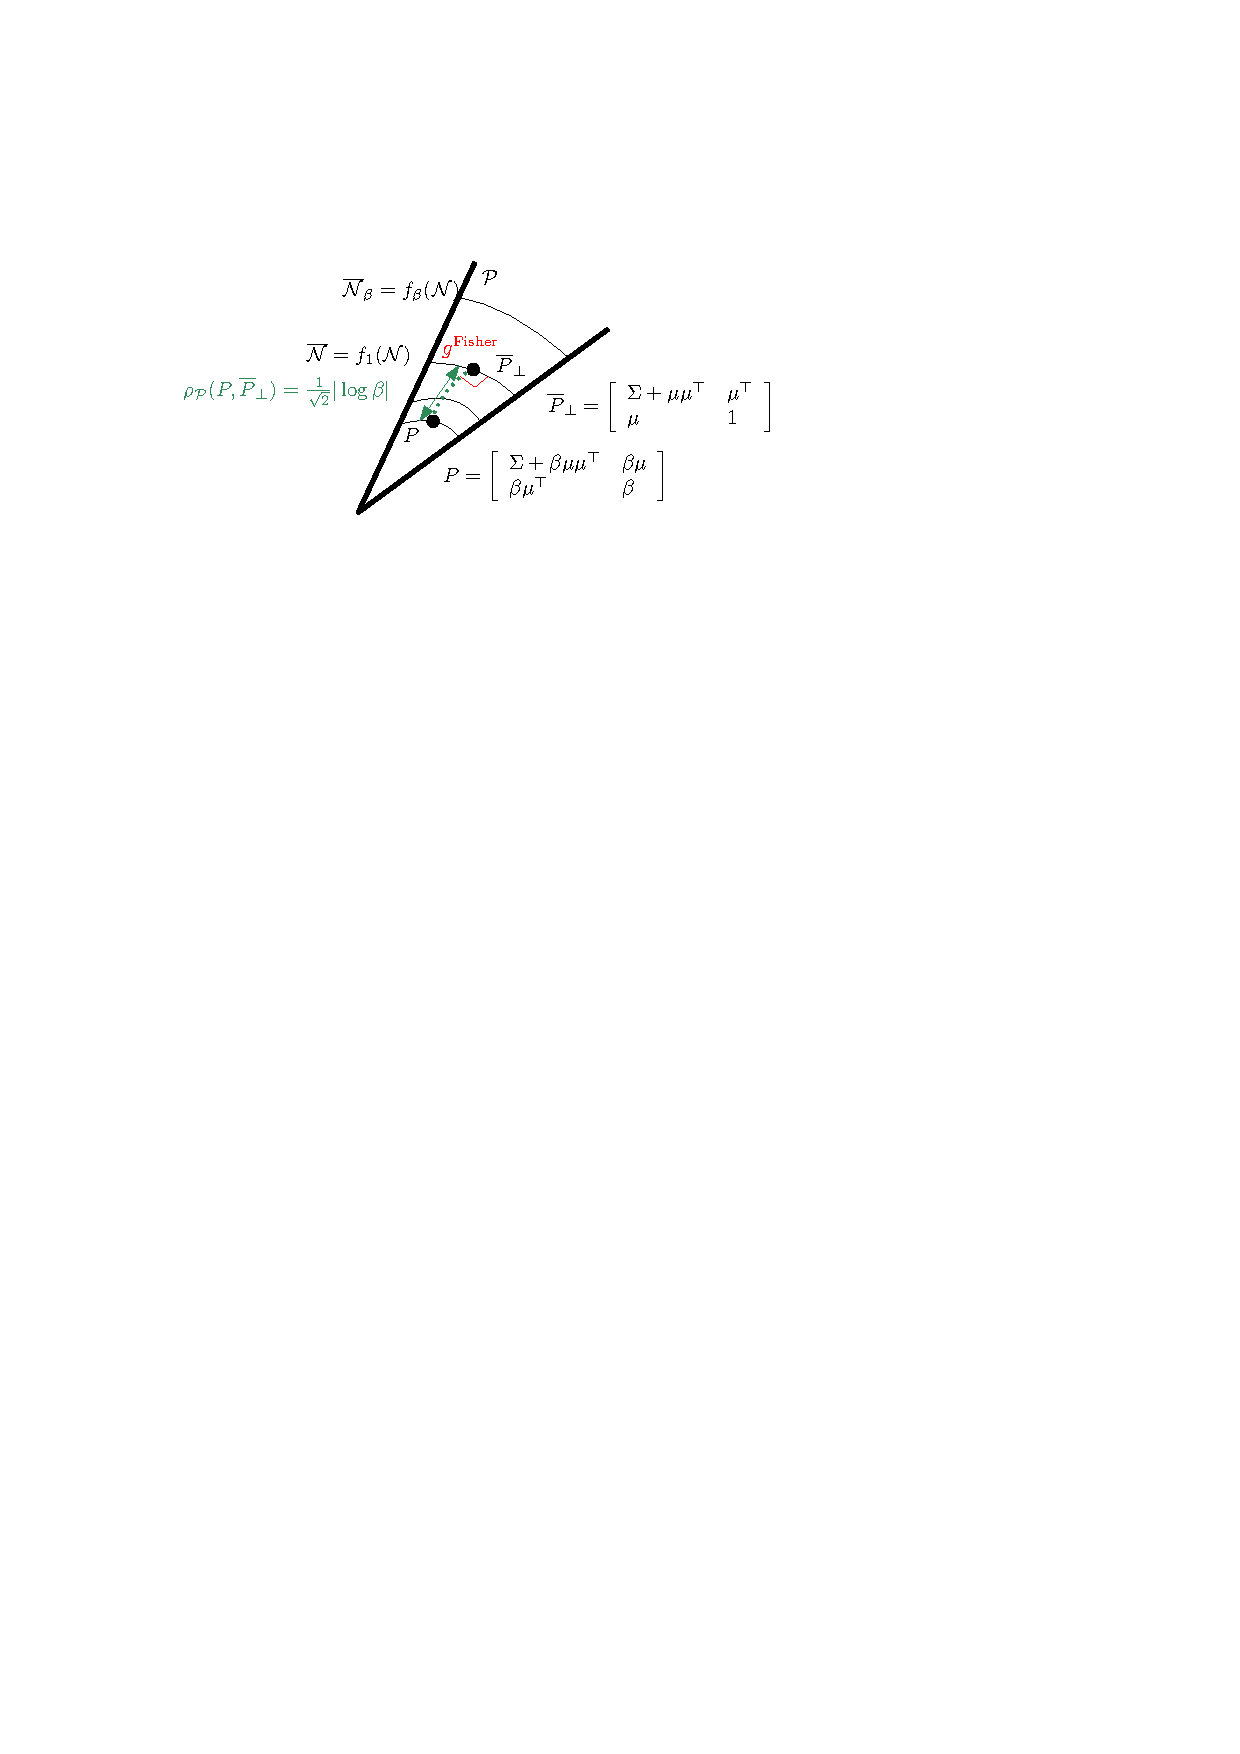
\includegraphics[width=0.65\textwidth]{FigIpe-OrthogonalProjectionSPD.pdf}

Here are some examples of the curves $c_\CO$ (in green) compared to the Fisher-Rao geodesics (in black):

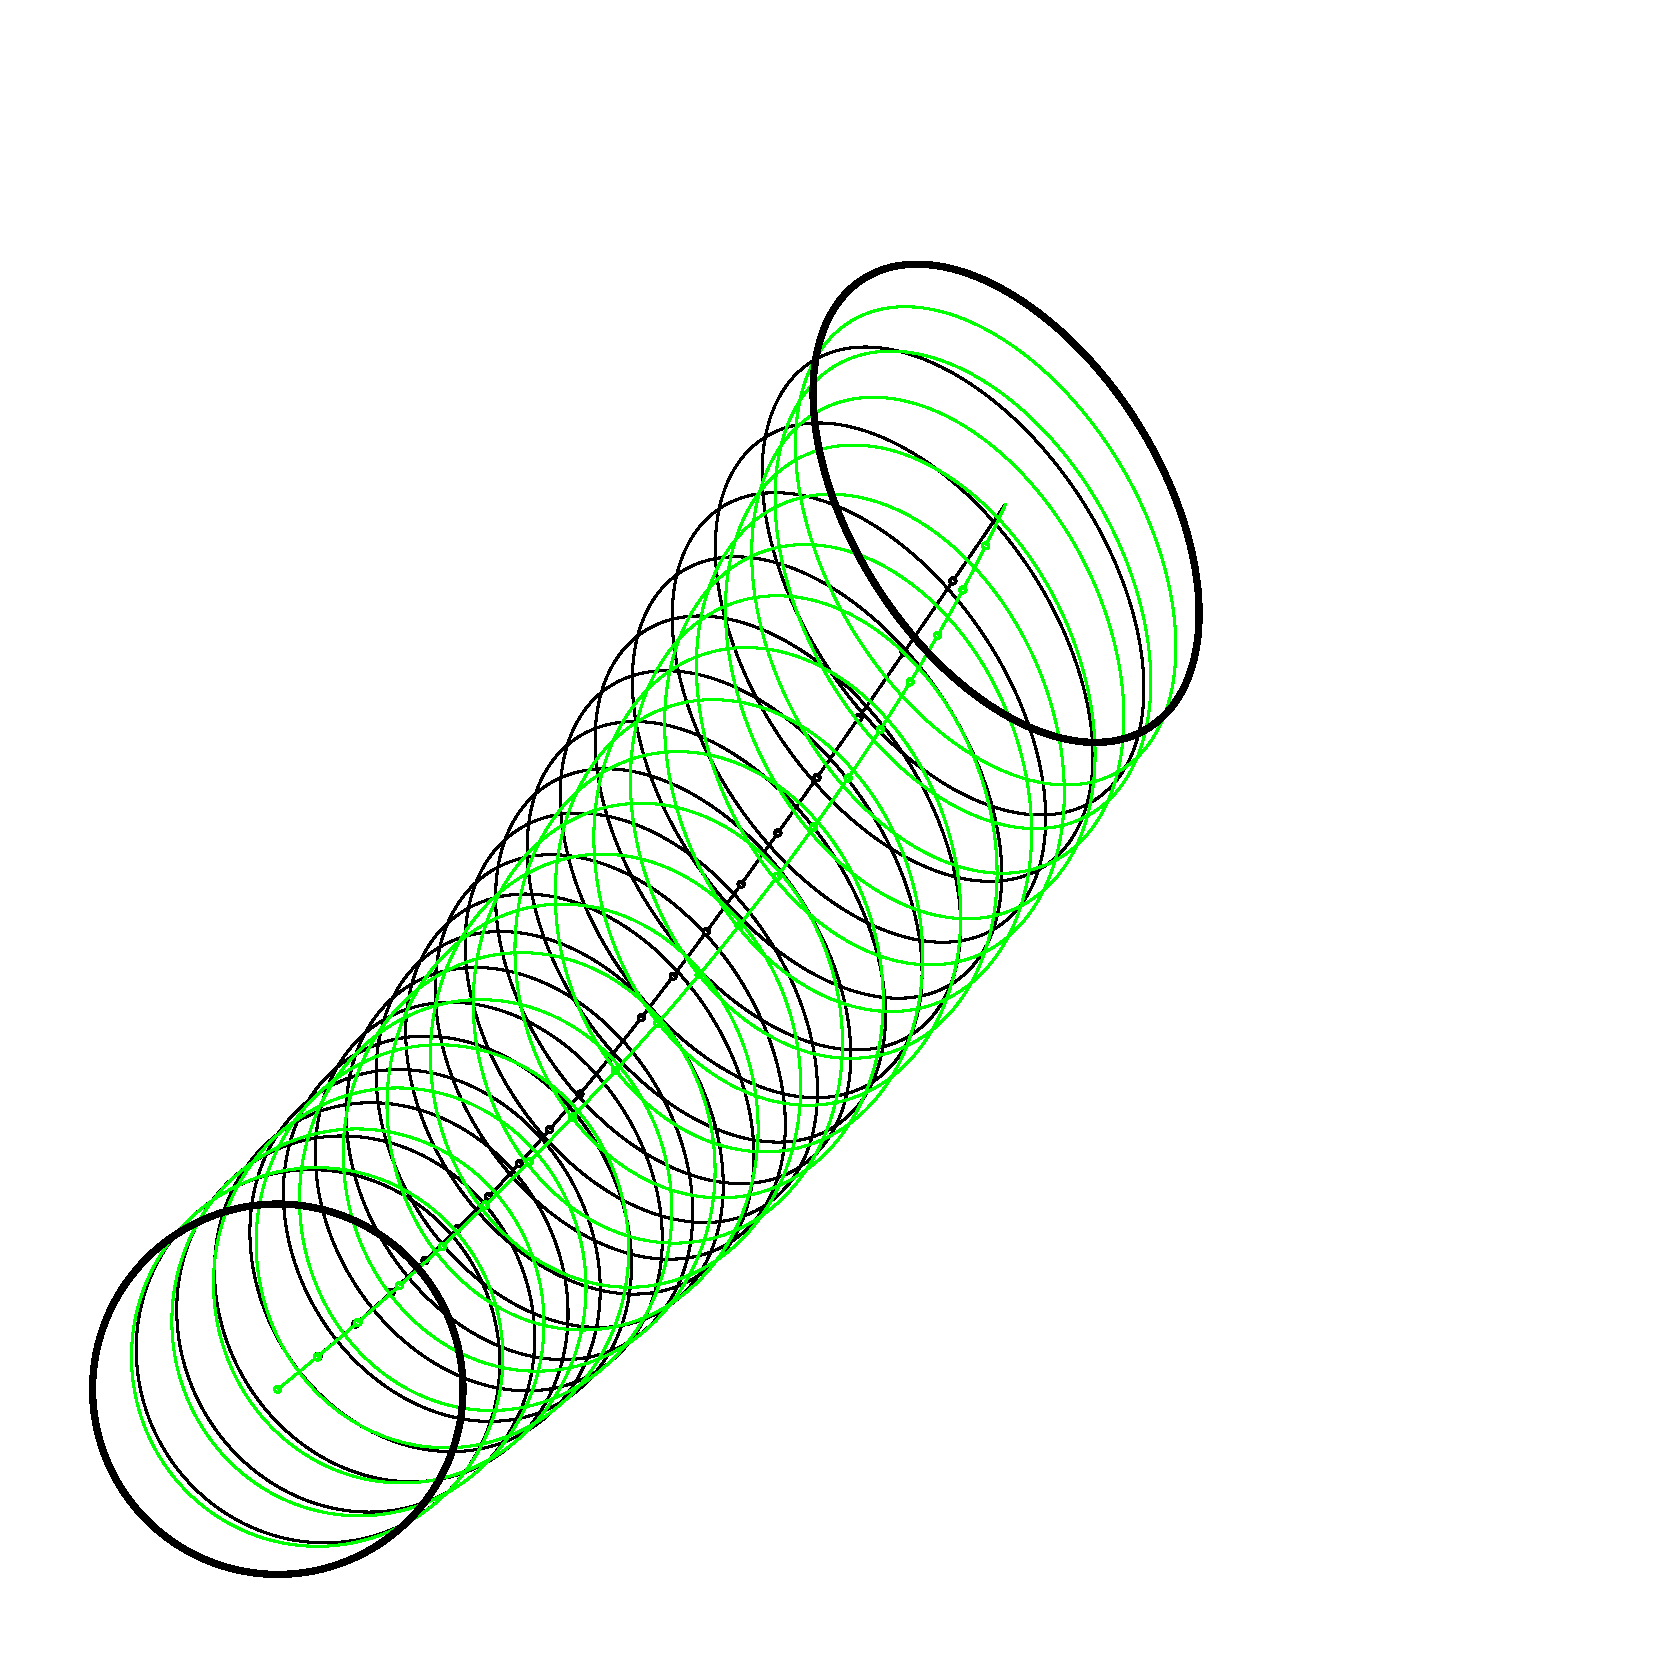
\includegraphics[width=0.65\textwidth]{BivariateNormal-11918040.pdf}


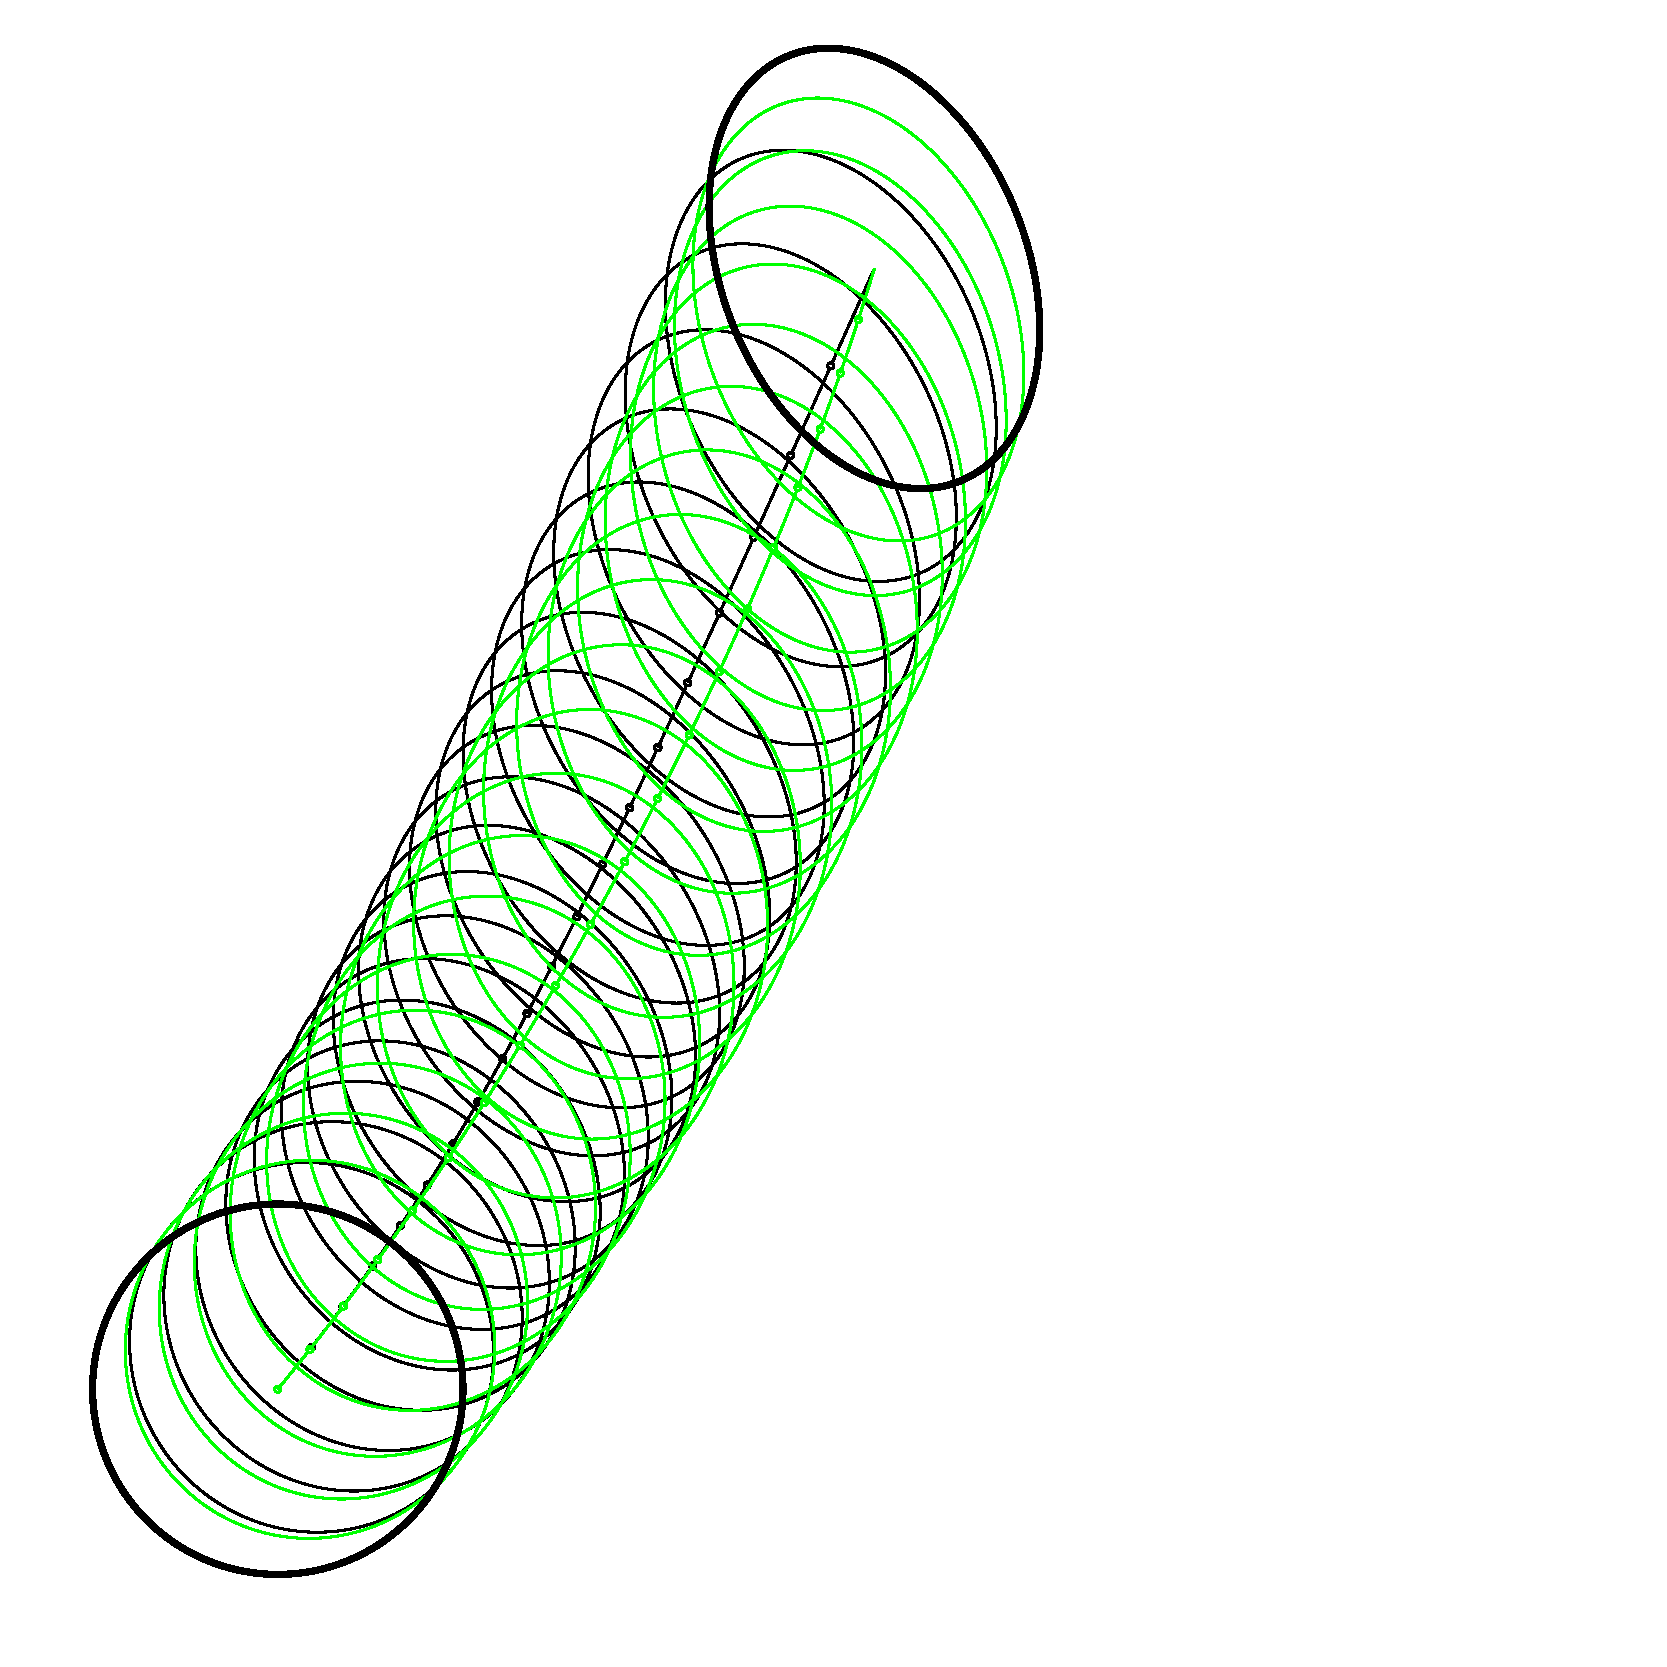
\includegraphics[width=0.65\textwidth]{BivariateNormal-11892050.pdf}


More details and quantitative analysis: \url{https://www.mdpi.com/1099-4300/25/4/654}

\end{document}